%Wf4ever Main Document File
\documentclass[a4paper, twoside, 11pt]{article}

\usepackage[scaled=0.92]{helvet}
\usepackage{fancyhdr}
\usepackage{courier}
\usepackage{caption}
\usepackage{subcaption}
%\usepackage{subfigure}
\normalfont % in case the EC fonts aren't available
\usepackage[T1]{fontenc}
\parskip=2pt\parindent 0pt


\usepackage{url}
\usepackage{listings}
\usepackage{inconsolata}
\usepackage{hyperref}
\usepackage{wf4ever}
\usepackage{xspace}
\usepackage{amsfonts}
\usepackage{amssymb}
\usepackage{amsmath}
\usepackage{verbatim}

\usepackage{color}
%figure with pdf latex
\usepackage[pdftex]{graphicx}
\usepackage{epstopdf}
\DeclareGraphicsExtensions{.jpg,.pdf,.png}

% Macros

% Identifying documents

\id{2.2v2}
\idyear{2013} %To adjust year for "Document Identifier"
\title{D\delid\ Design, implementation and deployment of workflow
  lifecycle management components - Phase II}
\coordinator{XX} %Del Coordinator
\institution{University of Manchester} %Del Coordinating Inst.
\authors{XX} %Other authors
\abstract{This deliverable describes the second phase of delivery of
  workflow lifecycle management components. It includes a description
  of the Research Object Model, which facilitates interoperation
  between components; an initial Research Object Storage and Retrieval
Service; RO Manager command line tool; and a definition of a model for
workflow abstraction.}
\version{0.1} %Please fill out version
\datesubmitted{June 1, 2013} %Submission date
\datedue{July 31, 2013} %Date due
\state{Draft} %State
\distribution{Public} %Distribution (Public, Restricted, Confidential)

\copyrighty{2013}



\begin{document}
\maketitle


\section*{Work package participants} The following partners have taken an active part in the work leading to the elaboration of this document, even if they might not have directly contributed to the writing of this document or its parts: %Enter Work Package Participants:
\begin{itemize}
\item iSOCO
\item OXF
\item PSNC
\item UNIMAN
\item UPM
\end{itemize}

\section*{Change Log}
%Fill in table
\begin{centering}

\begin{tabular}{|c|c|p{4.92cm}|p{6.5cm}|}

\hline \textbf{Version} & \textbf{Date} & \textbf{Amended by} & \textbf{Changes} \\ \hline
0.1 & 01-06-2013 & Khalid Belhajjame & Initial outline \\ \hline
%&&&\\ \hline
%&&&\\ \hline

\end{tabular}

\end{centering}
\clearpage
\section*{Executive Summary}
%Please enter Executive Summary
This deliverable describes the second phase of delivery of workflow
lifecycle management components. These components are focused around
the Wf4Ever Research Object Model (RO Model), which provides
descriptions of workflow-centric ROs -- aggregations of content. This
model is used to structure and describe ROs which are then stored and
manipulated by the components of the Wf4Ever Toolkit.

The RO Model provides a framework for describing aggregations of
content along with annotations of the aggregated resources, a
vocabulary for describing workflows, and a vocabulary for describing
provenance. The model underwent few changes in the last year in the light of user comments. 
We provide here a summary of the new version of the RO model.
We also present the components developed for creating and managing Research Objects: the
Research Object Storage and Retrieval API (implemented as part of the
Research Object Digital Library (RODL)) and a command line tool -- the
RO Manager. These components and services are also discussed in D1.2v3
(Wf4Ever Sandbox -- Phase II), D1.3v1 (Wf4Ever Architecture -- Phase
II) and D1.4v1 (Reference Wf4Ever Implementation -- Phase II). 

One of the main development in the last year consists in incorporating research objects within the myExperiment environment to allow scientists who already use myExperiment to create, share and reuse research objects. We discuss the efforts that went into this task, and report on an activity that we conducted to convert all existing Taverna T2 workflows into ROs.

We  present advanced management functions that we developed for abstracting and indexing workflows, with the aim of supporting the discovery and reuse of workflows. We present an ontology that we developed for abstracting workflows in terms of motifs that characterize data manipulation and transformation patterns, which we term motifs. We also report on a solution that we developed for indexing workflows based on the services (processes) that they use.

This deliverable should be read in tandem with D1.3v2 (Wf4Ever
Architecture -- Phase II), D1.4v2 (Reference Wf4Ever Implementation --
Phase II), D1.2v3 (Wf4Ever Sandbox -- Phase III), D3.2v2 (Design,
implementation and deployment of Workflow Evolution, Sharing and
Collaboration components -- Phase II) and D4.2v2 (Design,
implementation and deployment of Workflow Integrity and Authenticity
Maintenance components -- Phase II) in order to provide a complete
picture of the state of the Wf4Ever Phase II components.

\clearpage

\tableofcontents
\clearpage
\listoftables %Add comment to suppress list of tables
\listoffigures %Add comment to suppress list of figures

\clearpage
\sloppy

%Your work starts here

\section{Introduction}

\section{The Research Object Model}
\label{sec:romodel}

The design of the Research object model was informed by a systematic analysis of requirements expressed by scientists from the life sciences and astronomy fields. The results of such analysis are summarised in Figure \ref{fig:wm_abstract}, which distinguishes between core and extended requirements. There are three core requirements that have been identified, namely a mechanism for uniquely identifying Research Objects, a means for aggregating resources within a Research Object, and the ability to annotate the Research Object, its constituent resources and their relationships. Based on the core requirements, the extended requirements highlight the need for specifying workflows (experiments), provenance traces of their executions, the evolution of a Research object over time, as well as mechanisms for citing Research Objects, expressing their dependencies, etc.


\begin{figure}[ht]
  \centering
  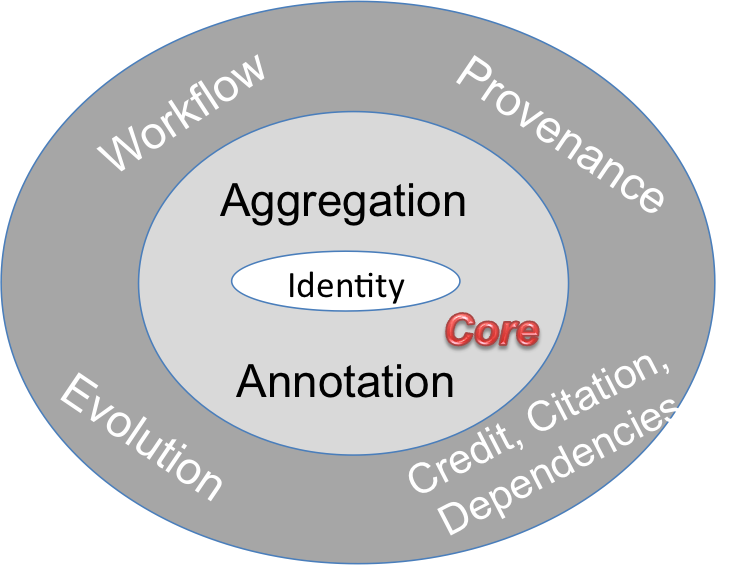
\includegraphics[width=0.4\textwidth]{Figures/wm_abstract.png}
  \caption{Research Objects: Abstract model.}
  \label{fig:wm_abstract}
\end{figure}

We have realized the Research Object abstract model illustrated in Figure \ref{fig:wm_abstract} in the form of a family of ontologies that are illustrated in Figure \ref{fig:wm_concrete}, which we will present in the rest of this section.  It is worth noting that some of the vocabularies, e.g., ORE\footnote{\url{www.openarchives.org/ore}} and OA ~\cite{COG11}, are existing vocabularies that we built on to specify our ontologies.

 \begin{figure}[ht]
  \centering
  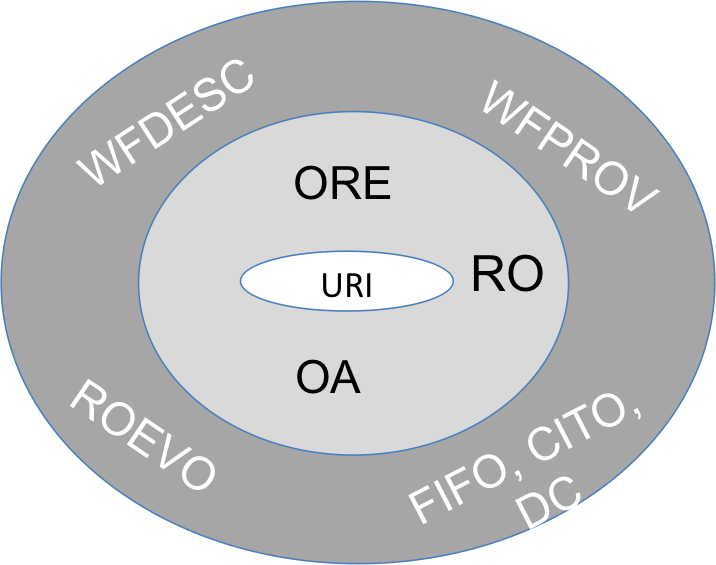
\includegraphics[width=0.4\textwidth]{Figures/wm_concrete.png}
  \caption{Research Objects: Concrete model.}
  \label{fig:wm_concrete}
\end{figure}

\subsection{RO core ontology} 
The Core RO Ontology provides the minimum terms that are essential to the specification of research objects. Specifically, it caters for two essential requirements by providing a container structure that can be used by the scientists to bundle the resources and material relevant for their investigation, and by enabling annotations of such a container, its resources, as well as the relationships between resources thereby making the research object interpretable and reusable. 

To cater for the specification of aggregation structures, we built the Research Object Core Ontology upon the popular ORE vocabulary. ORE defines standards for the description and exchange of aggregations of Web resources. 
Figure \ref{fig:ro_ontology} illustrates the main terms that constitute the Research Object Core Ontology, which we describe in what follows.


\begin{figure}[ht]
  \centering
  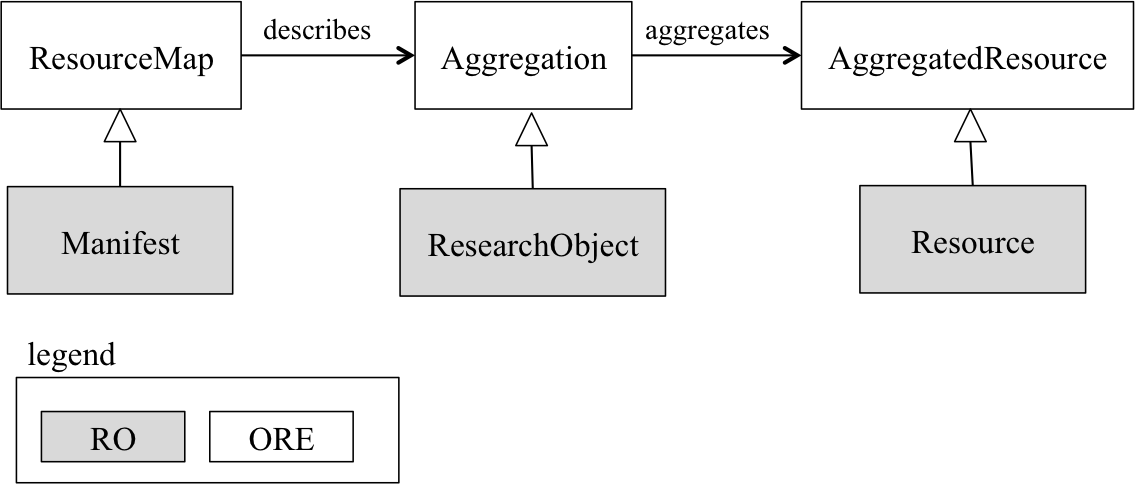
\includegraphics[width=0.6\textwidth]{Figures/ro_ontology_1.png}
  \caption{RO as an ORE aggregation.}
  \label{fig:ro_ontology}
\end{figure}

\begin{itemize}
\item
\texttt{ro:ResearchObject}\footnote{The namespace of the Research Object Core Ontology \texttt{ro} is \url{http://purl.org/net/wf4ever/ro\#}}, represents an aggregation of resources. It is a sub-class of \texttt{ore:Aggregation} and acts as an entry point to the research object.
\item
\texttt{ro:Resource}, represents a resource that can be aggregated within a research object and is a sub-class of \texttt{ore:AggregatedResource}. A resource can be a Dataset, Paper, Software or Annotation. Typically, a \texttt{ro:ResearchObject} aggregates multiple \texttt{ro:Resource}, and this relationship is specified using the property \texttt{ore:aggregates}.
\item
\texttt{ro:Manifest}, a sub-class of \texttt{ore:ResourceMap}, represents a resource that is used to describe a \texttt{ro:ResearchObject}. It plays a similar role to the manifest in a JAR or a ZIP file, and is primarily used to list the resources that are aggregated within the research object.
\end{itemize}

The second core requirement that, the Research Object Core Ontology caters for, is the descriptions of the research object and its elements. We chose the Annotation Ontology (AO) release 2.0b2~\cite{COG11}.To annotate research objects, we make use of the following three Annotation Ontology terms \texttt{ao:Annotation}\footnote{The namespace of \texttt{ao} is \url{http://purl.org/ao/}}, which represents the annotation itself; \texttt{ao:Target}, which is used to specify the \texttt{ro:Resource}(s) or \texttt{ro:ResearchObject}(s) subject to annotation; and \texttt{ao:Body}, which comprises a description of the target.
In the case of research objects, we use annotations as a mean for decorating a resource (or a set of resources) with metadata information. The body is specified in the form of a set of RDF statements, which can be used to, e.g., specify  the date of creation of the target or its relationship with other resources or research objects. Also, annotations can be provided for human consumption (e.g. a description of a hypothesis that is tested by a workflow-based experiment), or for machine consumption (e.g. a structured description of the provenance of results generated by a workflow run). Both kinds of annotations are accommodated using Annotation Ontology structures.

\subsection{RO Extension Ontologies}
We present in this section two  extensions to the core Research Object ontology. The first specializes the kinds of resources that the research object can aggregate. In particular, we present extensions to specify  method and experiments and the traces of their executions. The second kind of extension shows how specific metadata information, specifying the evolution of the research object over time, can be specified by specializing the Research Object core ontology.

\paragraph{Specifying Workflows}
To describe workflow research objects the workflow description vocabulary \textit{wfdesc}\footnote{The name space of \textit{wfdesc} is \url{http://purl.org/wf4ever/wfdesc\#}.} defines several specific resources that are involved in a workflow specification. The choice of these resources was performed by examining the commonalities between major data driven workflows, namely Taverna\footnote{http://www.taverna.org.uk}, Wings\footnote{http://http://wings-workflows.org} and Galaxy\footnote{http://galaxyproject.org}, to cite a few.

\begin{figure}[ht]
  \centering
  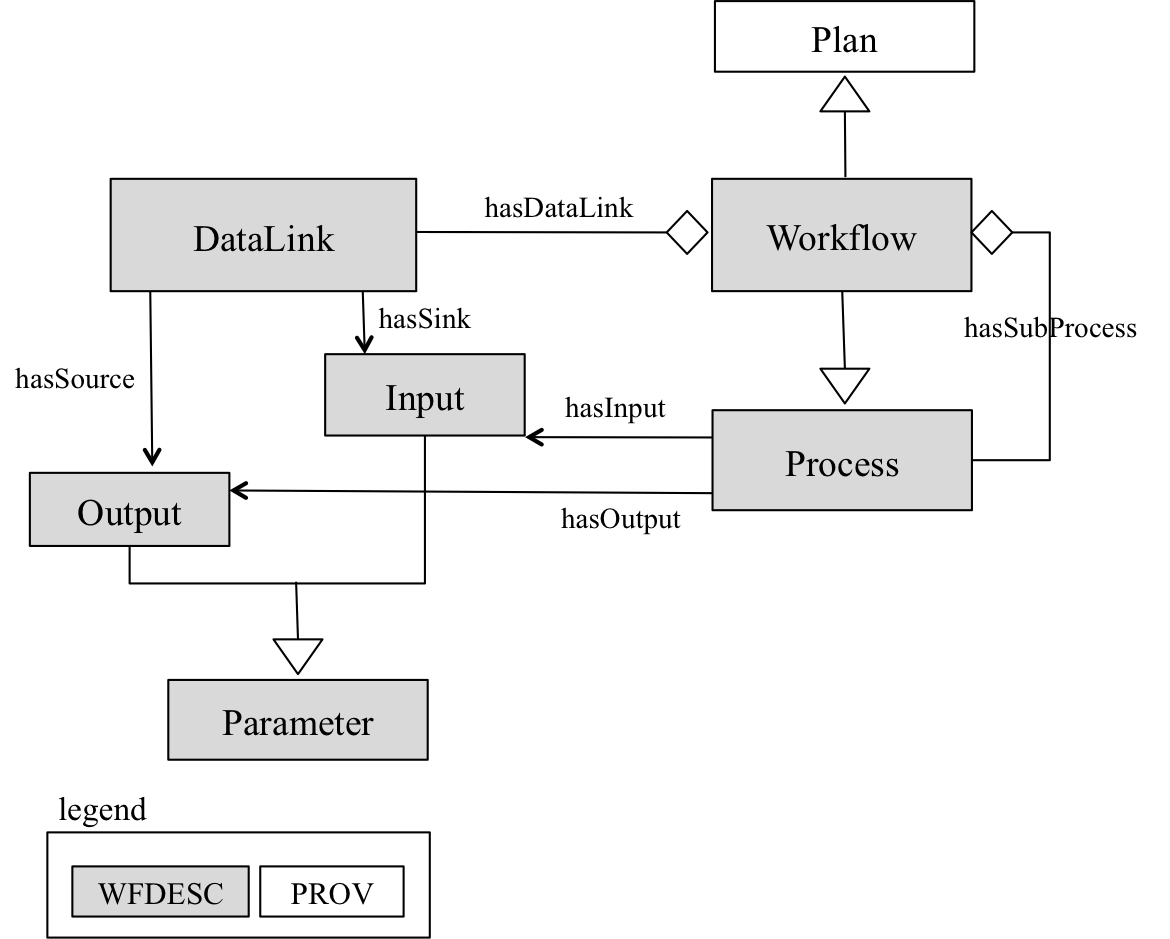
\includegraphics[width=0.6\textwidth]{Figures/wfdesc.png}
  \caption{The \textit{wfdesc} ontology.}
  \label{fig:wfdesc}
\end{figure}

Figure \ref{fig:wfdesc} illustrates the terms that compose the \textit{wfdesc} ontology. Using such ontology, a workflow is described using the following three main terms:
\begin{itemize}
\item
\texttt{wfdesc:Workflow} refers to a network in which the nodes are processes and the edges represent data links. It is defined as a subclass of the \textit{Plan} concept from the PROV-O ontology, which represents a set of actions or steps intended by one or more agents to achieve some goals \cite{w3c-prov-o}. 
\item
\texttt{wfdesc:Process} is used to describe a class of actions that when enacted give rise to process runs. Processes specify the software component (e.g., web service) responsible for undertaking those actions.
\item
\texttt{wfdesc:DataLink} is used to encode the data dependencies between the processes that constitute a workflow. Specifically, a data link connects the output of a given process to the input of another process, specifying that the artifacts produced by the former are used to feed the latter.
\end{itemize}


\paragraph{Describing Experimental Provenance using the \textit{wfprov} Vocabulary}
The \textit{wfprov} ontology is used to describe the provenance traces obtained by enacting  workflows. It is defined as an extension to the ongoing W3C PROV standard ontology - PROV-O\footnote{Note that the \textit{wfprov} is reported in the W3C PROV Working Group implementation report.}.

\begin{figure}[ht]
  \centering
  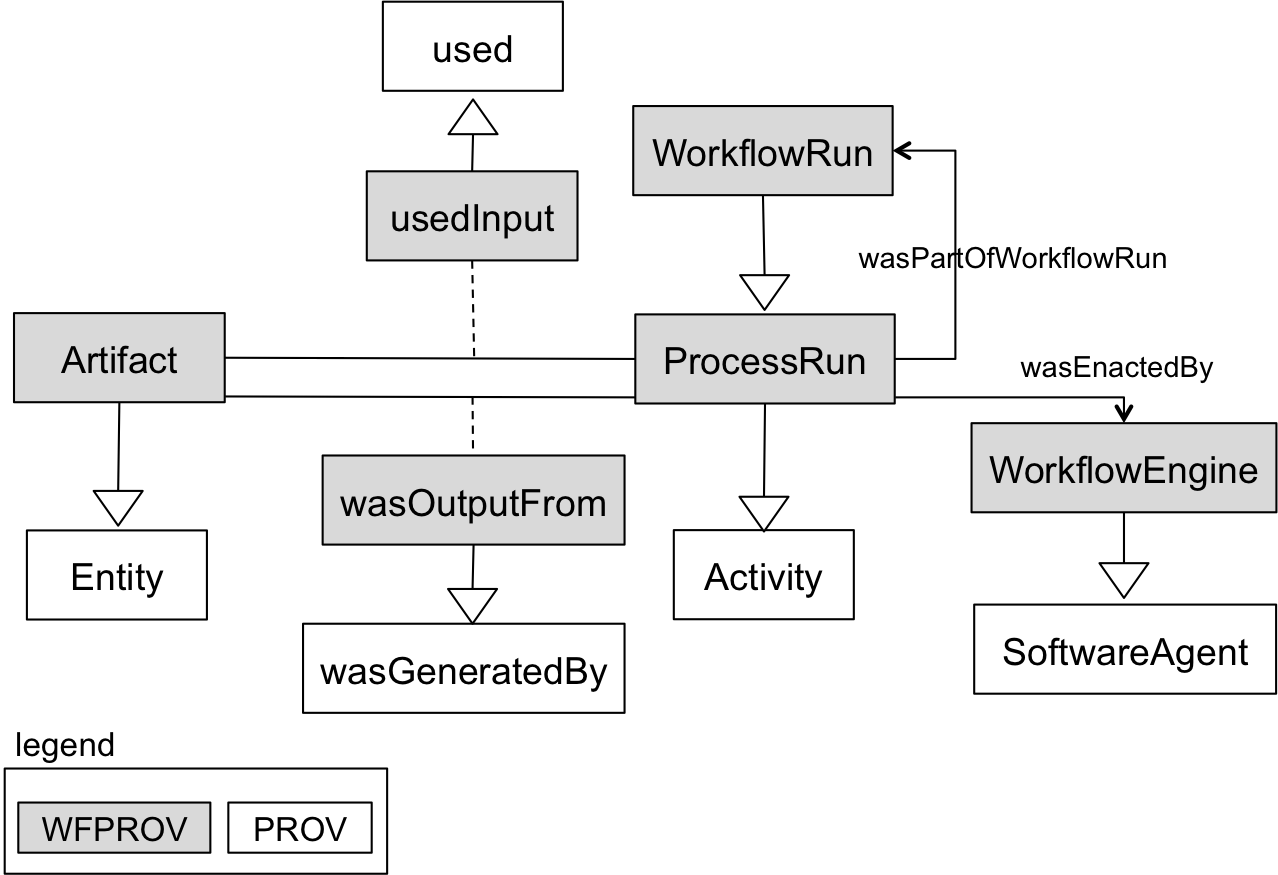
\includegraphics[width=0.6\textwidth]{Figures/wfprov.png}
  \caption{The \textit{wfprov} ontology.}
  \label{fig:wfprov}
\end{figure}

Figure \ref{fig:wfprov} illustrates the structure of the \textit{wfprov} ontology and its alignments with the W3C PROV-O ontology. A a workflow run~(\texttt{wfprov:WorkflowRun}) represents the enactment of a given workflow. It is composed of a set of process runs~(\texttt{wfprov:ProcessRun}), each representing the enactment of a process. A process run may use some artifacts~(\texttt{wfprov:Artifact}) as input and generate others as output. A process run is enacted by a workflow engine~(\texttt{wfprov:WorkflowEngine}), which can be seen as a PROV software agent.

By chaining the usage and generation of artifact together, the \textit{wfprov} ontology allows scientists to trace the lineage of workflow results. For example the user can identify the input artifacts that were used to feed the wokflow run (as a whole) to obtain a given output that was generated by the workflow run.

\paragraph{Tracking Research Object Evolution using the \textit{roevo} Vocabulary}
The \textit{roevo} ontology is another extension to the minimal core ontology for describing an important aspect of research objects, its life cycle.
%There are a number of existing work captures changes of information objects, like the changeset vocabulary, evolution of ontologies, like xxx, yyy, etc. 
To track the life cycle of a research object, we need to describe its changes at different levels of granularity, about the research object as a whole and about the individual resources. Also, we want to provide sufficient details to track the changes in order to roll back to a particular version or to quality control changes. Therefore, we need to describe when the change took place, who performed the change, and dependency relationships between the changes. %None of the existing vocabularies provide all the structure for us to build upon. 
Change is closely related to the provenance of a particular version of a research object or a resource. A study of the latest PROV-O ontology shows that it indeed provides all the foundational information elements for us to build the evolution ontology. 

\begin{figure}[ht]
  \centering
  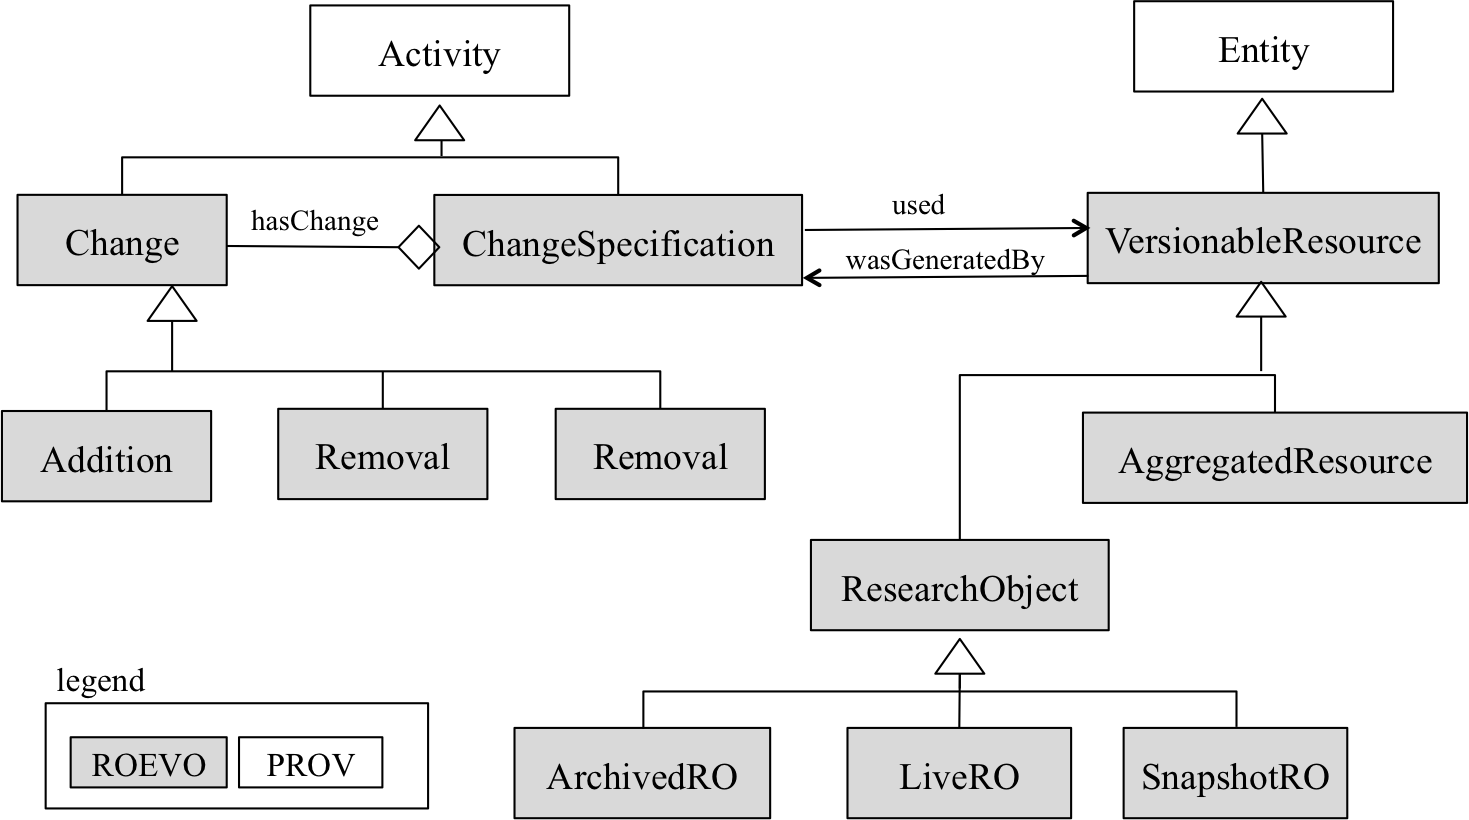
\includegraphics[width=0.6\textwidth]{Figures/roevo.png}
  \caption{The \textit{roevo} ontology extending PROV-O core terms.}
  \label{fig:ro_evo}
\end{figure}    

Figure~\ref{fig:ro_evo} illustrates the core concepts of this ontology and how it extends the PROV-O:
\begin{itemize}
\item To capture different status of a research object we create three sub-classes of \texttt{ro:ResearchObject}: the \texttt{roevo:LiveRO} is a research object to capture research findings during a live investigation and it can changed, and it can either archived or snapshotted. The \texttt{roevo:ArchivedRO} can be regarded as a production research object to be preserved and archived, such as one describing findings published in an article, and it can no longer be changed; the \texttt{roevo:SnapshotRO} represents a live Research Object at a particular time.
\item Both a snapshot of a live Research Object and an archived Research Object can be regarded as a versioned Research Object, i.e. a \texttt{roevo:VersionableResource}, Because it is a sub-class of \texttt{prov:Entity}, we can reuse PROV-O properties to describe the provenance or changes of this entity, such as pointing to the activity leading to any of its changes, the source research object that it was derived from, and the agent involved in its change.
\item A change is a \texttt{prov:Activity}, which means that it has a start time, an end time, an input entity and a resulting entity. Also a change leading to a new Research Object can constitute a series of changes. Therefore, we have a composite \texttt{roevo:ChangeSpecification} activity, which has a number of unit \texttt{roevo:Change}s. A unit change can be adding, removing or modifying a resource or a research object. But these different changes share the same pattern of taking an input entity and producing an output entity, which can all be nicely covered by properties from PROV-O.
\end{itemize}

As well as the above vocabularies, the Research Object model makes use of existing vocabularies, in particular, FOF\footnote{\url{http://xmlns.com/foaf/spec/}}, DCTerms\footnote{\url{http://dublincore.org/documents/dcmi-terms/}}, CITO\footnote{\url{http://vocab.ox.ac.uk/cito}}, and SCIOC\footnote{\url{http://sioc-project.org/ontology}} to provide Research Objects designers with the means to expresse aspects such as the people who were involved in the creation of a Research Object, its citation, as well as dependencies that the Research Object may have. For instance, we make use of the term \texttt{dc:requires} to specify that a the execution of a workflow requires other resources, e.g., plugins, credential, or specific execution environment.


\section{Research Object Storage and Retrieval}
This section presents the components that constitute the RODL, using a UML class diagram, and show how the user can utilize RODL using a UML sequence diagram.

\section{Research Object Manager}
This section presents the RO manager architecture, and presents the functionalities it provides using  a UML sequence diagram, if that is plausible. 

\section{Research Object-Enabled myExperiment}
This section describes the efforts that went into incorporating research objects within myExperiment. In particular, how the notion of myExperiment pack was used as a starting point to incorporate new features/functionalaities. We will also discuss the diferent iterations that involved Wf4ever and Biovel users in those developments.

\section{Workflow Abstraction using Motifs}
This section presents the motif ontology, again using a UML class diagram, and provides an example of a workflow that was annotated using the motifs.

\section{Workflow Indexation}
This section shows how workflows can be indexed using the trie structure. It presents the approach as well as an example workflow that is indexed.


\appendix
\clearpage
\addcontentsline{toc}{section}{Bibliography}
\bibliographystyle{alpha}
\bibliography{refs.bib}
%------------------------------------------------------------------------------------------------------
%Keep following label in order for Latex to get the total number of pages right
%---
\label{lastpage}
%---
\end{document}
